%% 
%% main.tex
%% Formatted NIP thesis conformed with the CS guidelines for the MS
%% Thesis and PhD Dissertation accepted for year 2005 onwards.
%% See nip.sty for possible modifications.
%%
%% Copyright (C) 2006  Johnrob Y. Bantang: johnrob.bantang@gmail.com
%%
%% This tex is free; you can redistribute it and/or modify it under
%% the terms of the GU General Public License as published by the
%% Free Software Foundation version 2. See gpl.txt.
%%
%% This tex files are distributed in the hope that it will be useful,
%% but WITHOUT ANY WARRANTY; without even the implied warranty of
%% MERCHANTABILITY or FITNESS FOR A PARTICULAR PURPOSE.  See the GNU
%% General Public License for more details.
%%
%% You should have received a copy of the GNU General Public License
%% along with this program; if not, write to the Free Software
%% Foundation, Inc., 51 Franklin Street, Fifth Floor, Boston, MA
%% 02110-1301, USA.
%%
%%
%%


\documentclass[bs]{nip3} %%use nip class
%% to add options: phd, ms, bs, applied
\usepackage[a4paper, total={6in, 9.25in}]{geometry}
%%packages to be used.
\usepackage[square,numbers,sort&compress]{natbib}
   %% square-bracketed, numbered, sorted, and compressed citations
   %% for more info: http://merkel.zoneo.net/Latex/natbib.php
\usepackage{verbatim} %% for \verbatiminput
\usepackage{graphicx} %% for the graphics environment
\usepackage[centertags]{amsmath}
\usepackage{amsfonts}
\usepackage{amssymb}
\usepackage{amsthm}
\usepackage{newlfont}
\usepackage{subfigure}
\usepackage{hyperref}

%% Header section
\title{Thesis Title} %%required
\author{Your Name} %% required
\email{Your email}%% appears only when draft version use \draft option.
\adviser{Adviser Name}{Ph.D.}%% required
\reader{First I. Reader}{Ph.D.}%% required
\secondReader{No A. Co-Adviser}{Ph.D.}%% optional if with coadviser
%\coadviser{Another A. Adviser}{Ph.D.}%% replace "\coadviser" with "\secondReader" if no co-adviser
\director{Wilson O. Garcia}{Ph.D.}%% required
\dean{Giovanni A. Tapang}{Ph.D.} %%required
\gradyear{2021} \gradmonth{July} %%graduation month and year
\defenseDate{xx June 2021}
\degreelevel{Bachelor of Science}
\course{Physics}

%% Preliminary pages' contents input here..
\dedication{ \input{dedication.tex} }%% optional, see dedication.tex for sample content.
\acknowledgments{ \input{acknowledgments.tex} } %% optional, see acknowledgment.tex for sample content.
\abstract{ This is where your abstract is!!!1 } %% see abstract.tex
\pacs{01.20.+x [Communication forms and techniques (written, oral,
electronic, etc.)], 01.30mm (Textbooks for graduates and
researchers)}

%% Main document section
\begin{document}
\maketitle %% creates title page, do not remove this line.
\makePrelim %% creates preliminary pages, do not remove this line.

% !TEX root =  main.tex
\chapter{Introduction}
\section{Background of Study}
\hspace{\parindent}


\section{Statement of the Problem}
\hspace{\parindent} 


\section{Objectives of the Study}
\hspace{\parindent} The study aims to investigate the effects of coherence in the performance of the phase retrieval algorithm specifically, the Single-Beam Multiple-Intensity Reconstruction (SBMIR). Through understanding the principles of speckle contrast and formation, and coherence, a model for the use of partially coherent illumination in SBMIR will be developed. Phase, as well as the amplitude, reconstructions will be analyzed throughout the investigation. The model will utilize a recently proposed enhanced SBMIR method that involves non-sequential propagation which addresses some issues of the conventional one. 

\section{Significance of the Study}
\hspace{\parindent}For years, partially coherent beams (PCB) have gained considerable attention because of their useful applications on different fields of optics and photonics. Compared to highly coherent beams, illumination from a partially coherent source reduces speckle effects and improves the image quality \cite{rayleigh}. These partially coherent light sources are found to be applied on free-space optical communications \cite{2020,chang}. Implementation using a partially coherent light source could extend the utilization and application of phase retrieval.

By introducing PCB light sources to the phase retrieval algorithm, specifically the intensity recording part, the configuration cost can be reduced significantly since they are more insensitive to external perturbations. The ability to maximize the available intensity measurements and information will make the proposed technique more cost-effective. Moreover, numerical simulations can provide valuable insights on a viable model for phase retrieval using partially coherent light.

\section{Scope and Limitation of the Study}
\hspace{\parindent}The reconstruction algorithms to be analyzed in this study are applied on numerically simulated intensity images. Reconstructions from experimental data are not in the scope of the study. In addition, the main basis for the OMW method is the Fresnel diffraction integral which was consequently used to simulate wave propagation. However, the Fresnel diffraction integral is known to scale with propagation distance and wavelength which limits the parameters that can be used in the numerical simulations [6]. Lastly, phase retrieval methods involving multiple intensity measurements are highly dependent on the intensity variations. Consequently, complete wave reconstruction cannot be always guaranteed as the reconstruction algorithm is object dependent as well.
% !TEX root =  main.tex
\chapter{Coherence Phenomenon}
\hspace{\parindent}
Light sources play significant roles on various optical processes and systems. Lights from known sources like lasers are nearly monochromatic and are known to be relatively coherent, while light from the sun is incoherent. The generated light beams from light sources of various degrees of coherence exhibit behaviors that are very different from one another. 

Coherence refers to the amount of correlation in the optical field at separate times or separate points within a beam of light \cite{Voelzbook}. High coherence leads to stationary interference effects such as the “fringing” and “ringing” structures that appeared in the simulated diffraction and imaging results for monochromatic (coherent) light \cite{Voelzbook}.

To be able to discuss coherence, it is convenient to first discuss classify coherence into two: temporal and spatial coherence. 

\section{Interference}
\hspace{\parindent} 




\section{Spatial Coherence}



\section{Temporal Coherence}



\section{Coherent Light}






\section{Incoherent Light}







\section{Partially-coherent Light}
% !TEX root =  main.tex
\chapter{Phase Retrieval}

This is a customized chapter.

\section{First section}

\hspace{\parindent} You may change the filename of this file as
long as you correspondingly change the filename stated in the
\verb+input{}+ line in the \verb+main.tex+.

\section{Including figures}

\hspace{\parindent} Figures can be added into your \LaTeX files
using the \verb+figure+ environment.  However, it is
\textbf{recommended} that you use \verb+.eps+ file format.  These
are encapsulated postscript files.  This can be easily done by
installing a postscript printer that outputs to a file (port is
FILE).  Ask your system administrator to install such a device for
producing \verb+eps+ files by simply printing it to that device.

Shown in Fig.~\ref{fig:sampleFig} is a figure created from
Excel\circledR. Note that the bounding box and page bounding box
should be adjusted well enough to show the correct field.
\begin{figure}[h]
  \centering %%used to center the figure
  %% The width option is used to rescale the figure into the proper
  %% fraction of the \columnwidth
  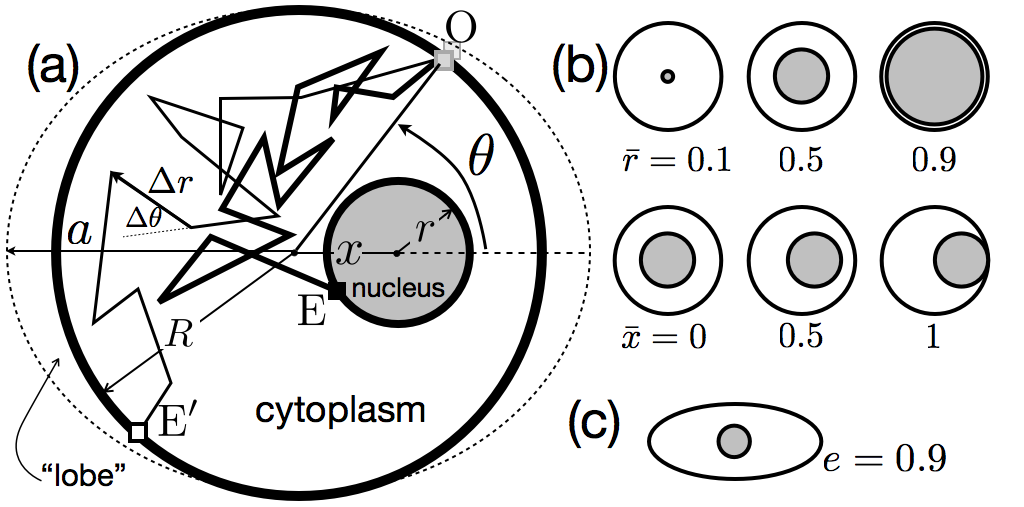
\includegraphics[width=0.8\columnwidth]{figures/model.png}\\
  \caption{
  A *.png file.
  }\label{fig:sampleFig}
\end{figure}

Please see the sample chapter on how the figure is included in the
\verb+tex+ files.
 %%could be model or experiment set-up
% !TEX root =  main.tex
\chapter{Results and Discussion}

In this chapter, a sample for making equations and sub-equations
are demonstrated.

\section{Equations and sub-equations}

\hspace{\parindent} In the following, a set of equations is shown.
\begin{subequations}
\newcommand\del{\overrightarrow{\nabla}}
\begin{equation}\label{eq:EGauss}
    \del \cdot \vec{D} = \rho
\end{equation}
\begin{equation}\label{eq:BGauss}
    \del \cdot \vec{B} = 0
\end{equation}
\begin{equation}\label{eq:Faraday}
    \del \times \vec{E} = -\partial_t \vec{B}
\end{equation}
The last one being
\begin{equation}\label{eq:Ampere-Maxwell}
    \del \times \vec{H} = \vec{J} + \partial_t \vec{D}
\end{equation}
\end{subequations}
Note that text can still be placed between sub-equations within
the \verb+subequations+ environment.

When using a solitary equations, you may use the usual equation
syntax in \LaTeX.
\begin{equation}\label{eq:Maxwell}
    E = mc^2
\end{equation}

%% The next lines are to demonstrate the items in the Bibliography. 
\nocite{stein} 
\nocite{AppliedOptics}
\nocite{HandbookOfOptics2} %%could be results and discussions
\input{5summaryAndConclusions.tex}
%% you may add more chapters by including more files just as above.
%% see the files for patterns of the format used.

\appendix
\input{appendix.tex}

\bibliographystyle{plain}
\bibliography{biblio} %% see file: "biblio.bib"
\addcontentsline{toc}{chapter}{Bibliography}

\end{document}
%%end of main.tex
